\documentclass[xcolor=svgnames]{beamer}
\mode<presentation>{}
\usetheme{CambridgeUS}
\usepackage{soul}%for using the strikethrough
\usepackage{url}%for using underscore
\usepackage{minted}%for using code blocks
\usepackage{lmodern}% for using different SVG colors
\newcommand\Fontvi{\fontsize{30}{7.2}\selectfont}
\setbeamertemplate{navigation symbols}{}
\setbeamercolor{block}{bg=Lavendar, fg=Maroon}
\title{Web Development using Ruby on Rails}
\author{Vysakh Sreenivasan}
\institute[vysakh.quora.com]{
  Submify.com\\
  vysakh.quora.com\\[1ex]
  \texttt{vysakh0 - twitter/facebook} 
}
\date{March 24, 2013}

\begin{document}
\AtBeginSection[]
{
  \begin{frame}{Table of Contents}
    \tableofcontents[currentsection, currentsubsection]

  \end{frame}
}
\begin{frame}[plain]
  \titlepage
  \begin{center}
    
\includegraphics[width=0.5\textwidth]{ruby-on-rails1.jpg}
  \end{center}
\end{frame}
\section{Introduction to Ruby}
\begin{frame}
\transwipe
  \begin{center}
    
\includegraphics[width=0.5\textwidth]{ruby.png}
  \end{center}
\end{frame}
\subsection{Why Ruby?}
\begin{frame}{Why Ruby?}
\transwipe
  \Fontvi
  \uncover<2->{\textcolor{DarkCyan}{be} \textcolor{Maroon}{productive}} \\
  \bigskip
  \bigskip
  \hspace*{3.5cm}\textcolor{DarkCyan}{enjoy} \textcolor{Maroon}{programming} \\
  \bigskip
  \bigskip
  \uncover<3->{\textcolor{DarkCyan}{be} \textcolor{Maroon}{happy}}
\end{frame}
\subsection{Features}
\label{sub:Features}
\begin{frame}[fragile]{HELLO WORLD}
\transwipe
  \transboxout
  \begin{minted}{c}
    #include<stdio.h>

    int main(){
      printf(``Hello World'');
      return 0;
    }
  \end{minted}
\end{frame}
\begin{frame}[fragile]{HELLO WORLD}
 \begin{minted}{java}
    import java.io.*;

    public class Example {

      public static void main(String[] args) {
      System.out.println(``Hello World'');
      }

    }
  \end{minted}
\end{frame}

\begin{frame}[fragile]{Simplicity}
\transwipe
\begin{columns}[c]
    \column{1.5in}
\begin{alertblock}{Ruby}
  \begin{minted}{ruby}
    puts ``Hello World''
  \end{minted}
\end{alertblock}
    \column{3in}
\uncover<2->{\begin{center}
  
\includegraphics[width=0.5\textwidth]{jacky.jpg}
\end{center}}
\end{columns}
\end{frame}
\begin{frame}
\transwipe
  \begin{itemize}
	  \item \alert<+>{Easy to Learn}
	  \item \alert<+>{Open Source}
	  \item \alert<+>{Rich libraries}
	  \item \alert<+>{Truly Object Oriented}
	  \item \alert<+>{Less Coding with fewer bugs}
	  \item \alert<+>{Helpful Community}
\end{itemize}
\end{frame}
\subsection{Getting Started}
\begin{frame}[fragile]
\transwipe
\begin{columns}[c]	
  \column{1.5in}
\begin{itemize}
  \item[] \alert<+>{}
  \vfill\item \alert<+>{Interactive Ruby}
  \vfill\item \alert<+>{Simple Syntax}
  \vfill\item \alert<+>{Variables}
    \begin{itemize}
      \vfill\item \alert<+>{Naming Convention}
    \vfill\item \alert<+>{Constants}
    \end{itemize}

\end{itemize}
\column{2.5in}
  \begin{overprint}
    \onslide<2>
    \begin{block}
      {Type small bits of ruby code, see it get executed}
   \end{block}
    \onslide<3>
    \begin{block}
      {Parenthesis, Braces, Tab spaces- Optional}
    \end{block}
    \onslide<4>
    \begin{minted}{ruby}
      a = 5
      b = 10
      c = a + b
      d = 11.4
      word = ``Cool :)''
    \end{minted}
    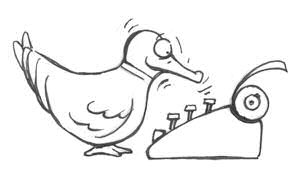
\includegraphics[width=0.5\textwidth]{duck.jpg}
    \onslide<5>
     \color{DarkCyan}{%
       \st{Camel Case} \\
       \st{firstName = ``vysakh''} \\
     }
     \color{Crimson}{%
       \url{first_name = ``Vysakh''}
     }
    \onslide<6>
    \begin{minted}{ruby}
      Pi = 3.14

      #Constants begin with Capital letter
    	
    \end{minted}
    \end{overprint}
\end{columns}
\end{frame}
\begin{frame}
\transwipe
\Fontvi
\color{Maroon}{In Ruby, everything is}
\begin{center}
  
\includegraphics[width=0.5\textwidth]{object.png}
\end{center}
\end{frame}
\begin{frame}[fragile]
\transwipe
\begin{columns}[c]	
  \column{1.5in}
  \begin{itemize}
    \item \alert<+>{Logical Operators}
    \item \alert<+>{Loops} 
    \item \alert<+> {List} 
    \item \alert<+>{Hash and Sybmols}
    \item \alert<+>{Functions}
    \item \alert<+>{Classes}
  \end{itemize}

  \column{2.5in}
  \begin{overprint}
    \onslide<1>
      \begin{minted}{ruby}
	
	if 1 == 1
	 puts ``1 is equal to 1''
	
	elsif 1 != 1
	 puts ``1 is not equal to 1''
	
	else
	puts ''Something else``
	end
      \end{minted}
  \onslide<2>
    \begin{itemize}
    	\item for
	\item while
	\item times
	\item upto
	\item downto
	\item step
	\item until
    \end{itemize}
    \onslide<3>
      \begin{minted}{ruby}


	numbers = [1, 3, 55, 2999]
	
	fruits = [''Mango``, ''Apple``]
	
	mixed = [1, ''Mango``]
      \end{minted}
      \onslide<4>
      \begin{minted}{ruby}
	
	
	names = {''first`` => ''Mark``} 

	#Strings are expensive

	# ``first'' is a string
	# :first is a symbol
	
	names = {:first => ''Mark``}
      \end{minted}
      \onslide<5>
      \begin{minted}{ruby}
	def add a, b
	 a+b
	end

	puts add 1, 2
      \end{minted}

      \onslide<6>
      \begin{minted}{ruby}
      class Calc

      def add a, b
       a+b
      end
      
      end

      class ChildCalc < Calc
      end

      c = Calc.new
      puts c.add 4, 5
      child = ChildCalc.new
      puts child.add 3, 4
    \end{minted}

    \end{overprint}
\end{columns}
\end{frame}
\subsection{Installation}

\begin{frame}[c]{Installation}
\transwipe
  \textbf{Use Ruby Version Management Tool} \\
  \bigskip
  \begin{center}
  \uncover<2->{\Fontvi \color{Maroon}{RVM or rbenv}}
  \end{center}
\end{frame}

\section{Introduction to Rails}
\begin{frame}
\transwipe
  \begin{center}
    
\includegraphics[width=0.5\textwidth]{rails.jpg}
  \end{center}
\end{frame}

\subsection{Why Rails?}
\label{sub:Why Rails?}
\begin{frame}{Why Rails?}
  \begin{itemize}
 \item \alert<+>{Extremely Productive Web Framework } 
 \item \alert<+>{Develop 10 times faster than a Java Framework }
 \item \alert<+>{Rails promotes best practises } 
 \item \alert<+>{Rails is very mature web framework }
 \item \alert<+>{Open Source, Vibrant Community }
 \item \alert<+>{Access to hundreds of gems }

  \end{itemize}
	
\end{frame}
\begin{frame}{Rails Philosophy}
  \begin{itemize}
  	 \item \alert<+>{Convention over Configuration}
	 \item \alert<+>{Donot Repeat Yourself (DRY)}
	 \item \alert<+>{REST is the best pattern for web applications }
	
  \end{itemize}
  \begin{center}
  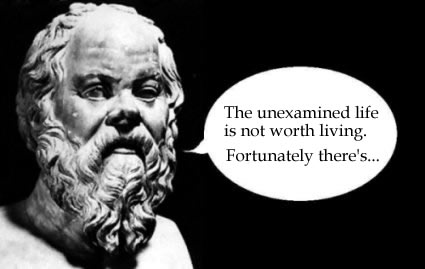
\includegraphics[width=0.5\textwidth]{socrates.jpg}	
  \end{center}
\end{frame}
\begin{frame}{FULL STACK FRAMEWORK.. WHAT??}
  \color{Maroon}{It abstracts and manages all parts of a web application}
	\begin{itemize}
		 \item \alert<+>{Database(model) }
		 \item \alert<+>{HTML/visualization(view) }
		 \item \alert<+>{Request flow(Controller) }

	\end{itemize}
\end{frame}
\subsection{MVC Pattern}
\begin{frame}{MVC Pattern}
\transwipe
  \begin{center}
  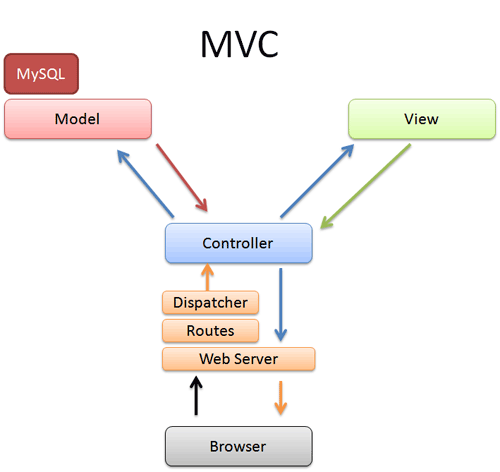
\includegraphics[width=0.5\textwidth]{rails-mvc.png}
  \end{center}
\end{frame}

\begin{frame}{Model}
\transwipe
  \begin{itemize}
   \item \alert<+>{Maps a table in the database with a ruby object}
 \item \alert<+>{Validates your data before saving them}
 \item \alert<+>{Here you manipulate your data}
 \item \alert<+>{Here you add associations}	
  \end{itemize}
\end{frame}
\begin{frame}{Controller}
\transwipe
	\begin{itemize}
	 \item \alert<+>{Each method is a function that your application exposes}
	 \item \alert<+>{Controls the flow of the request}
	 \item \alert<+>{Exposes your data to views}
	\end{itemize}
\end{frame}
\begin{frame}{Views}
  Show data to the user (in various format: html, csv, pdf..)
\end{frame}

\begin{frame}{Routes}
It is a map between the HTTP request and the method of a controller
\end{frame}
\begin{frame}{Migration}
  \begin{itemize}
    \item {add column/remove column}
	   \item {rename column/rename table}
	   \item {change column}
	   \item {create table/drop table}
  \end{itemize}
	
\end{frame}
\subsection{Ruby utilities}
\begin{frame}[fragile]{Rake}
\transwipe
    Rake a simple ruby build program with capabilities similar to make.
    \begin{itemize}
      \item Create a file Rakefile \\
    \end{itemize}
    \begin{minted}{ruby}
      namespace :my do
      task :alarm do
       puts ``Turned off alarm.''
      end
      end
      \end{minted}
      \begin{itemize}
      	\item Run this rake file with the command \textbf{rake my:alarm}
      \end{itemize}
 	
\end{frame}
\begin{frame}{gem and bundler}
\transwipe
  \begin{description}
    \item[gem]{A RubyGem is a software package, commonly called a gem. Gems contain a packaged Ruby application or library.} \\
    \item[bundler]{Bundler is the way to manage gem dependencies in Rails}
  \end{description}
	
\end{frame}
\subsection{Installation}
\begin{frame}{Installation and Creation}
  \begin{description}
    \item[Installing]{gem install rails}
    \item[Creation]{rails new project}
  \end{description}
\end{frame}
\subsection{REST}
\begin{frame}{What is REST?}
\transdissolve
\begin{center}
    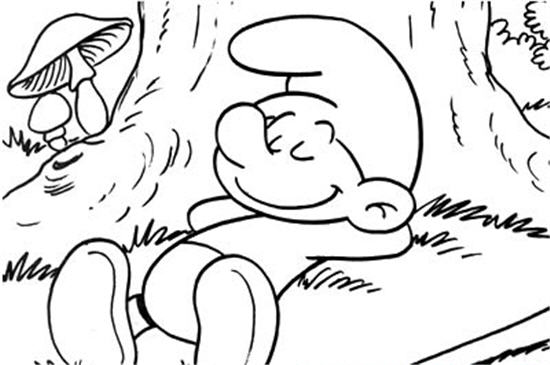
\includegraphics[width=0.5\textwidth]{rest.jpg}
	\end{center}
\end{frame}
\begin{frame}{Representational State transfer}
  REST in terms of Rails boils down to two main principles:
	\begin{itemize}
		\item Using resource identifiers such as URLs to represent resources.
		 \item Transferring representations of the state of that resource between system components.

	\end{itemize}
	
\end{frame}
\begin{frame}[fragile]{Rest - Example}

For example, the following HTTP request: DELETE /photos/17 \\
would be understood to refer to a photo resource with the ID of 17, and to indicate a desired action:  deleting that resource. \\
\begin{description}
	\item[In config/routes file] resources :photos
\end{description}
	\textbf{In controller}
	\begin{minted}{ruby}
	  class PhotosController < ApplicationController

	  def destroy
	  end
	  
	  end

	\end{minted}

	
\end{frame}
\section{Notes}
\subsection{Installation}
\begin{frame}{Installation}
	\begin{description}
	  \item[rbenv]{https://github.com/sstephenson/rbenv}
	  \item[RVM]{http://beginrescueend.com/}
	  \item[Windows]{http://railsinstaller.org/}

	  \item[Mac]{http://mxcl.github.com/homebrew/}
	\end{description}
\end{frame}
\subsection{Tutorials}
\label{sub:Tutorials}
\begin{frame}{Tutorials}
  \begin{block}{Ruby}
  	\begin{itemize}
	  \item \url{http://tryruby.org/}
  	\end{itemize}
  \end{block}
  \begin{alertblock}{Rails}
  	
    \begin{description}
      \item[Getting Started with Rails] \url{http://guides.rubyonrails.org/getting_started.html}
      \item[Michael Hartl's Book]\url{http://guides.rubyonrails.org/getting_started.html}
      \item[Rails Zombies]\url{http://railsforzombies.com/}
    \end{description}
  \end{alertblock}
  \begin{block}{Rails Reference}
    \textbf{Railscasts} \url{http://railscasts.com/}
  \end{block}
\end{frame}
\subsection{Help}
\label{sub:Help}
\begin{frame}{Help}
\begin{description}
  \item[Mailing list] \url{http://groups.google.com/group/rubyonrails-talk}
\item[StackOverflow] \url{http://stackoverflow.com/}
\end{description}
\end{frame}
\begin{frame}{Start Coding! :)}
  \begin{center}
    
\includegraphics[width=0.5\textwidth]{faster.jpg}
  \end{center}
\end{frame}

\end{document}
